\documentclass{beamer}
\usepackage[utf8]{inputenc}
\usepackage[T1]{fontenc}
\usepackage{lmodern}
\usepackage{graphicx}
\usepackage{amsmath, amssymb, graphicx}
\usepackage{listings}
\usepackage{color}
\usepackage{subcaption}

%\usepackage{beamerthemeshadow}
%\beamersetuncovermixins{\opaqueness<1>{25}}{\opaqueness<2->{15}}
\usetheme{Ilmenau}
\begin{document}
\title{Free Surface Flows} 
\date{03.02.2014}
\author{M. Farahani, E. Wolter, A. Hahn}
\frame{\titlepage}
%\frame{\frametitle{Structure}\tableofcontents} 


\section[Problem]{Problem description} 
%\subsection{}
\frame{ %\frametitle{ } 
Finde eine st\"uckweise zwei mal stetig differenzierbare Bahnkurve der Hinterachse $\Phi \in C^1([0,t^*],\mathbb{R}^2)$, sodass\\
\begin{enumerate}[(I)]
\item das Auto zu jedem Zeitpunkt $t$ in einem Gebiet $G$ ist
\item die Randbedingungen f\"ur $\Phi(0), [\Phi(t^*)]_2$ erf\"ullt sind und
  $\frac{\Phi'(0)}{\|\Phi'(0)\|} = \frac{\Phi'(t^*)}{\|\Phi'(t^*)\|} =\begin{pmatrix}-1 \\ 0 \end{pmatrix}$
\item f\"ur $-\frac{\Phi^{'}(t)}{\| \Phi^{'}(t) \|_2} = \begin{pmatrix} \cos \beta(t)\\ \sin \beta(t) \end{pmatrix}$\\
$\beta(t) \in \left[0, \frac{\pi}{2}\right[ \mbox{f\"ur alle  } t \in \left[0,t^*\right]$ erf\"ullt ist
\item (Wendekreisbeschr\"ankung erf\"ullt)
  
\end{enumerate}
}
\section{Free Surface Flow} 
\subsection{Application}

\begin{frame}
 		\begin{figure}
 			\begin{subfigure}[c]{0.3\textwidth}
 		 	      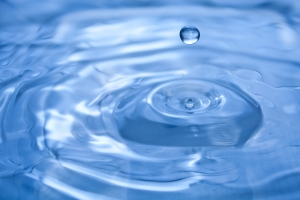
\includegraphics[width=1\textwidth]{pic/images.jpg}
 		 	\end{subfigure} 		 	
 		 	 \begin{subfigure}[c]{0.3\textwidth}
 		 	      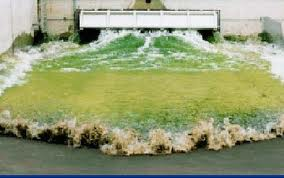
\includegraphics[width=1\textwidth]{pic/images1.jpg}
 		 	\end{subfigure}
 		 	
 		 	\vspace{1em}
 		 	
 			\begin{subfigure}[c]{0.3\textwidth}
 		 	      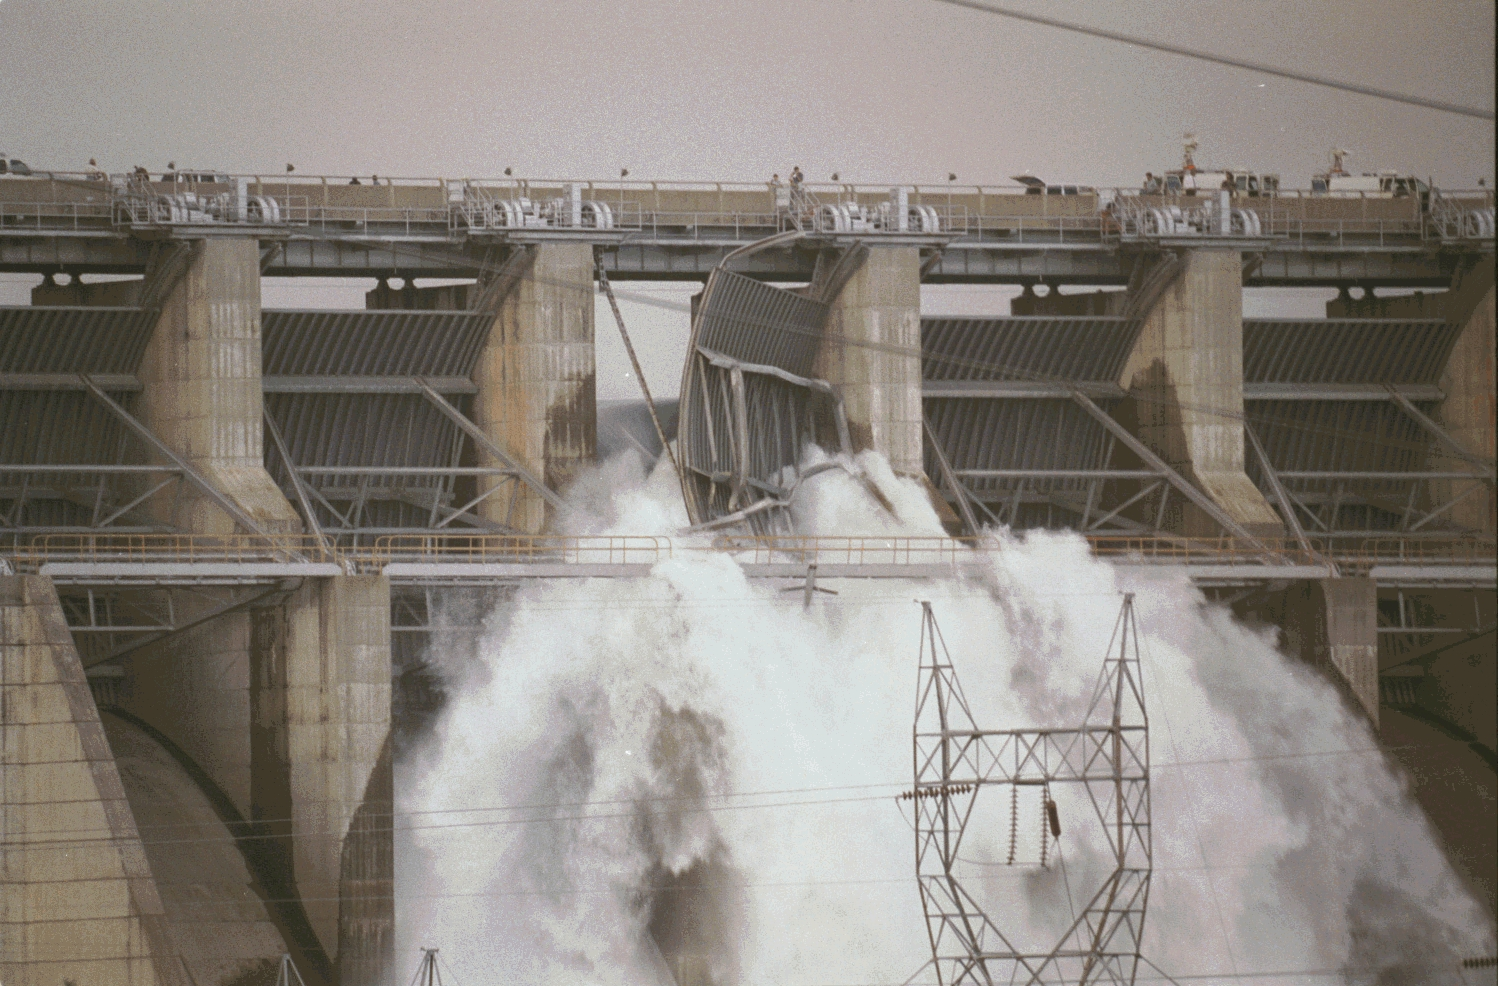
\includegraphics[width=1\textwidth]{pic/images2.jpg}
 		 	\end{subfigure}
 		 	 \begin{subfigure}[c]{0.3\textwidth}
 		 	      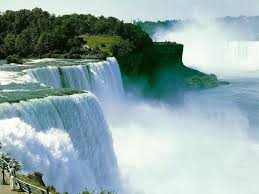
\includegraphics[width=1\textwidth]{pic/images3.jpg}
 		 	\end{subfigure}   
 		\end{figure}
\end{frame}	

\subsection{Theory}
	\begin{frame}{One empty neighbor}
		\begin{figure}
			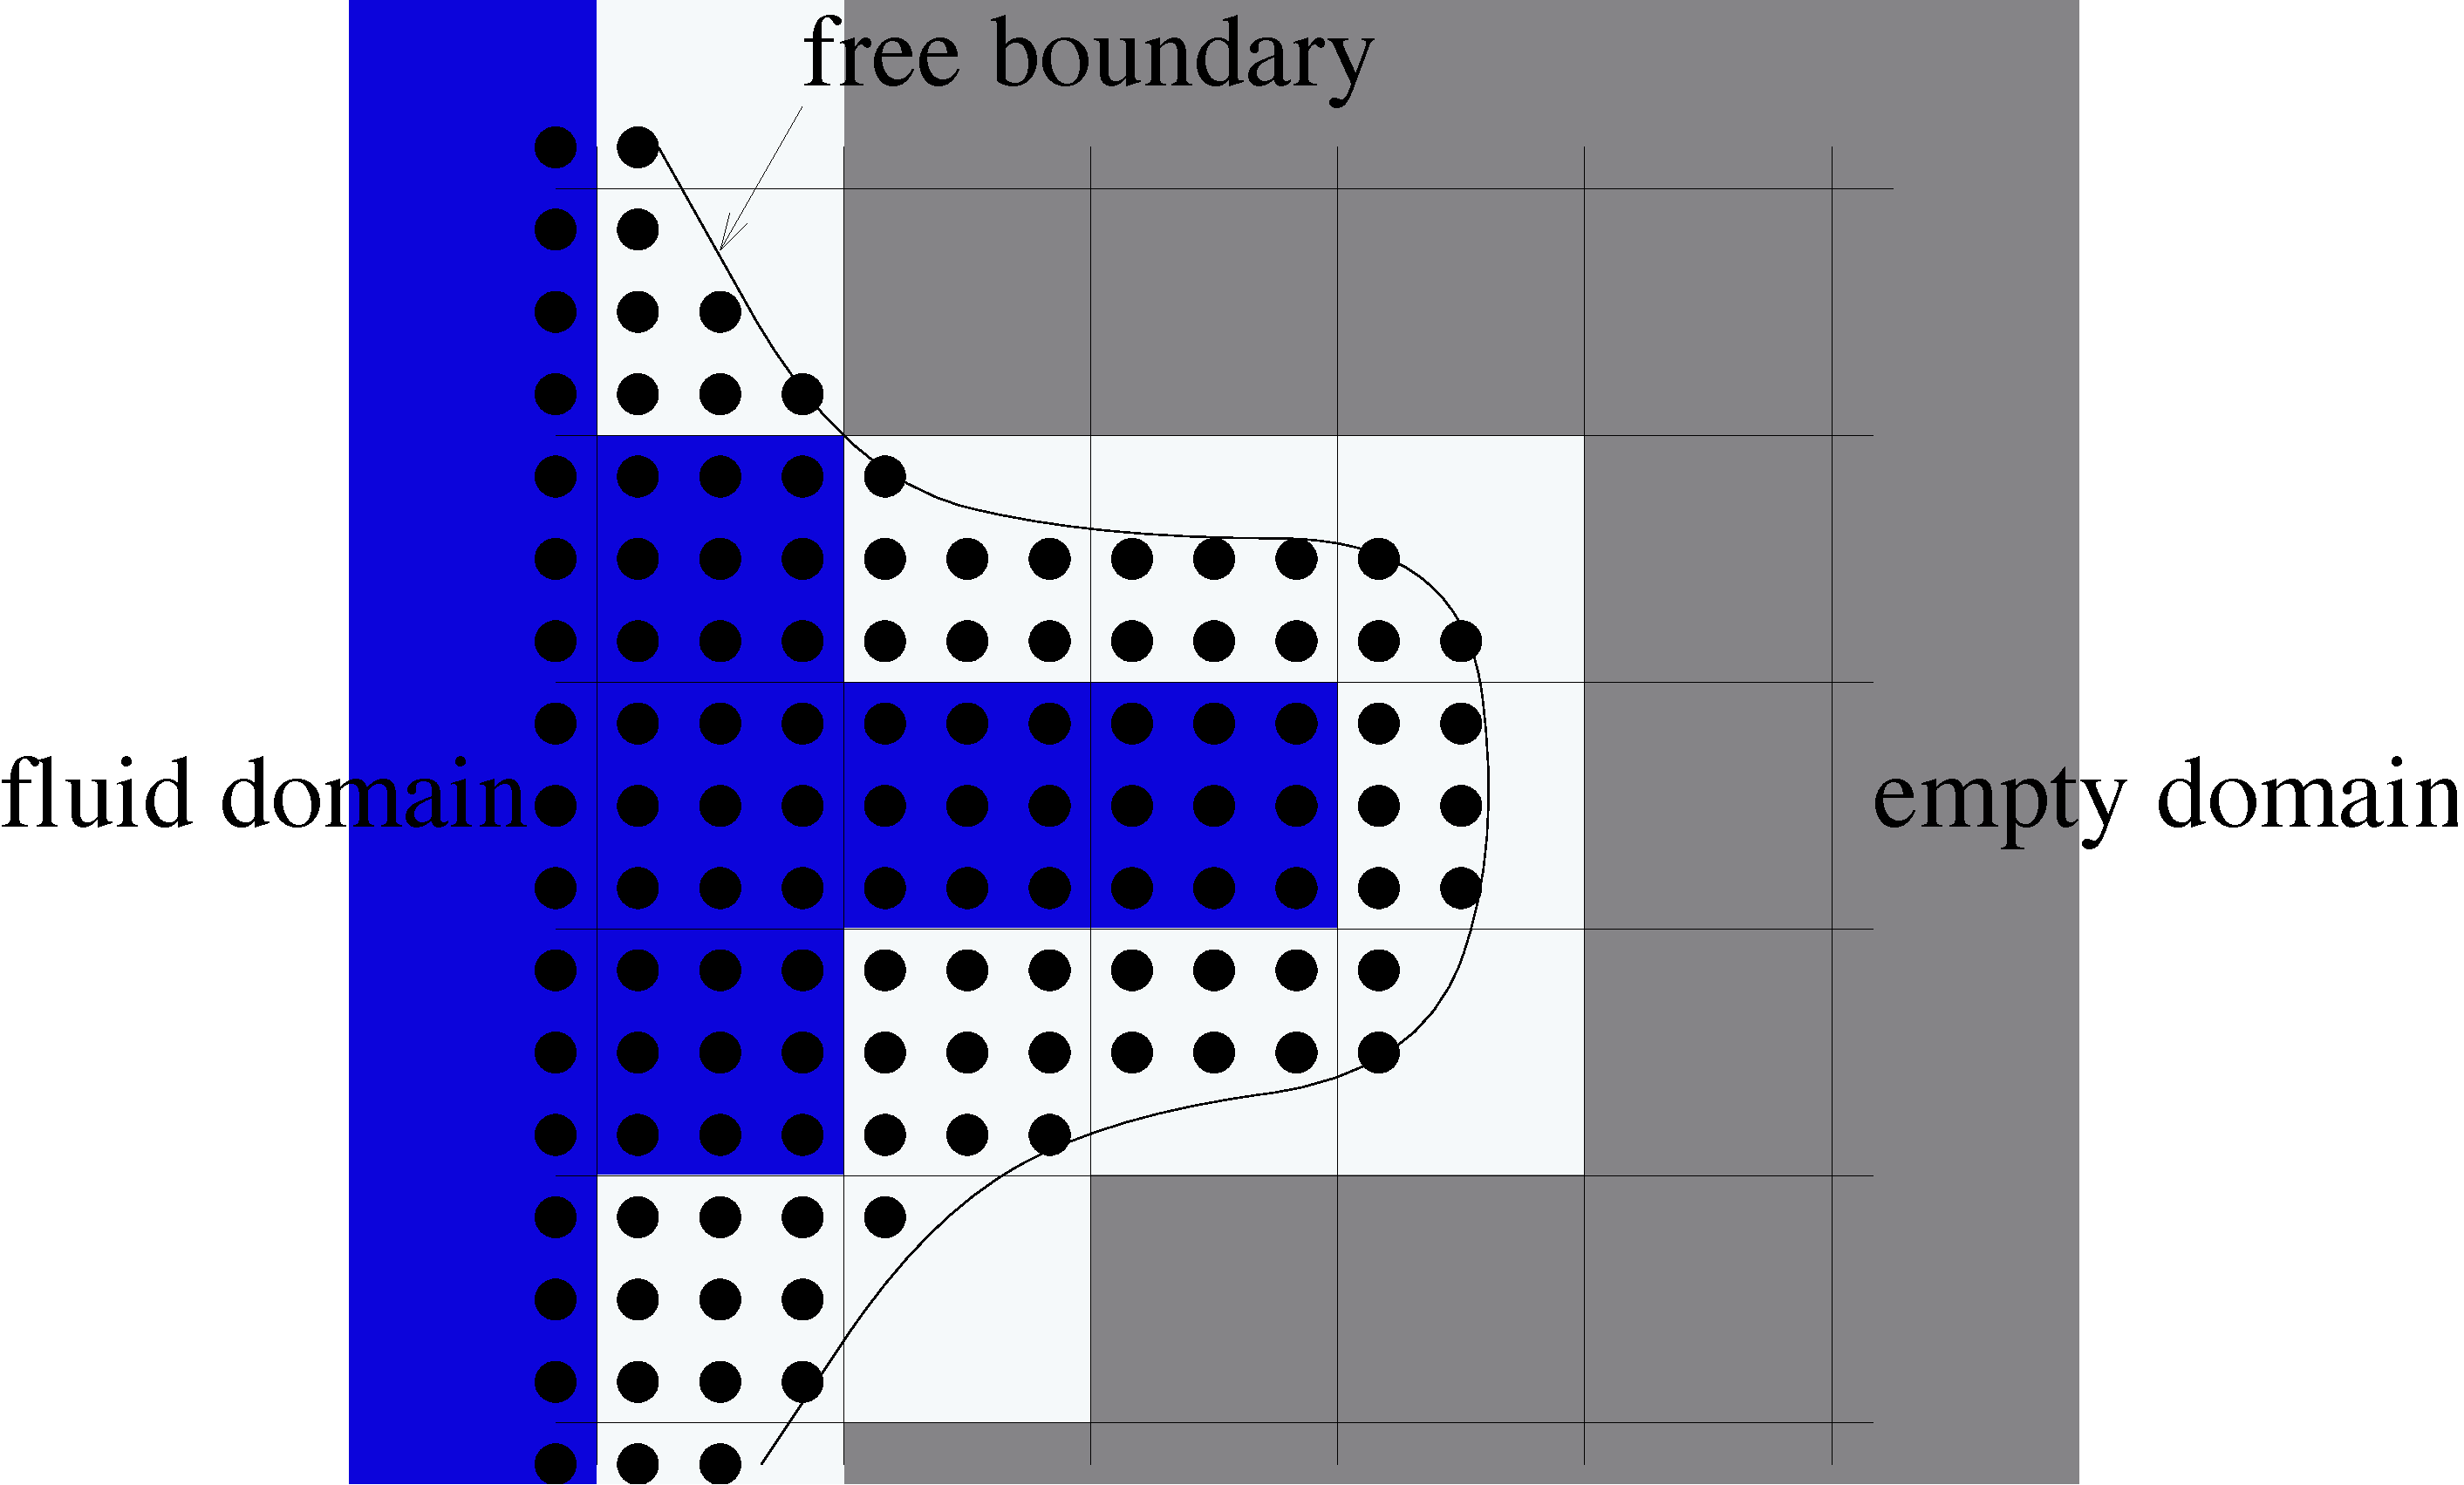
\includegraphics[width=1\textwidth]{pic/all.pdf}
		\end{figure}
	\end{frame}	

\subsection{Free surface treatment}
	\begin{frame}{One empty neighbor}
		\begin{figure}
			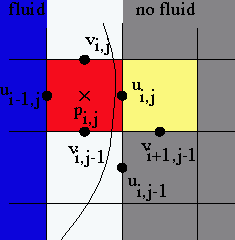
\includegraphics[width=1\textwidth]{pic/one.pdf}
		\end{figure}			
		
	\end{frame}	
	
	\begin{frame}{Two empty neighbor-common corner}
			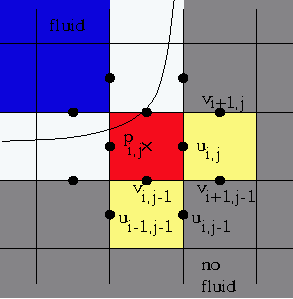
\includegraphics[width=0.49\textwidth]{pic/two1.pdf}

	\end{frame}	
	
	\begin{frame}{Two empty neighbor-opposite side}
			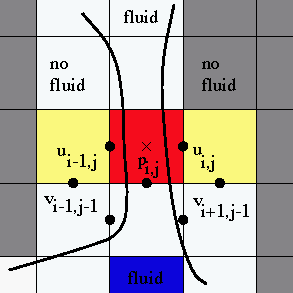
\includegraphics[width=0.49\textwidth]{pic/two2.pdf}

	\end{frame}	
	
	\begin{frame}{Three empty neighbor}
			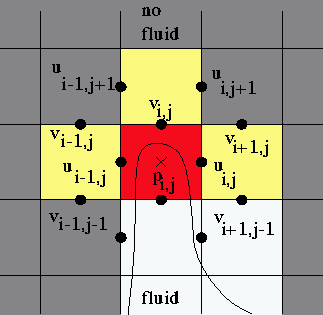
\includegraphics[width=0.49\textwidth]{pic/three.pdf}
	\end{frame}	
		
	\begin{frame}{Four empty neighbor}
			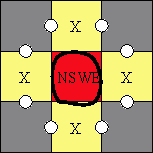
\includegraphics[width=0.49\textwidth]{pic/four.pdf}

	\end{frame}	 	
\section{Implementation} 
\subsection{Creating New Code}
\frame{\frametitle{Particle and ParticleTracer}
\begin{itemize}
\item \textbf{Particle(real x, real y, int type)} \\
Has some functions which can detect its position on the grid
\item \textbf{ParticleTracer(StaggeredGrid *grid)} \\
Has a vector of particles
\begin{itemize}
\item \textbf{void markCells()}
\item \textbf{void fillCell(int i, int j, int numParticles, int type)}
\item \textbf{void addRectangle(real x1, real y1, real x2, real y2, int type)}
\item \textbf{void addCircle(real x, real y, real r, int type)}
\item \textbf{void advanceParticles(real const dt)}
\end{itemize}
\end{itemize}
}

\subsection{Changing Old Classes And Functions}
\frame{\frametitle{Types and StaggeredGrid}
\begin{itemize}
\item \textbf{Types.hh}:
\begin{itemize}
\item \textbf{flag EMPTY}
\end{itemize}
\item \textbf{StaggeredGrid.cc}:
\begin{itemize}
\item \textbf{int ppc\_}
\item \textbf{bool isEmpty(const int x, const int y)}
\item \textbf{void setCellToEmpty(int x, int y)}
\item \textbf{void refreshEmpty()}
\end{itemize}
\end{itemize}
}
\frame{\frametitle{FluidSimulator}
\begin{itemize}
\item \textbf{FluidSimulator.cc}:
\begin{itemize}
\item \textbf{real rectX1\_particle\_, rectX2\_particle\_ , ...}
\item \textbf{real circR\_particle\_, circX\_particle\_, ...}
\item \textbf{void set\_UVP\_surface(int i, int j , const real \&dt, bool compP)}
\item \textbf{void one\_empty\_neighbour(int i , int j , const real \&dt, bool compP)}
\item ...
\item \textbf{four\_empty\_neighbour(int i , int j , const real \&dt, bool compP)}
\item \textbf{void refreshEmpty()}
\end{itemize}
\end{itemize}
}

\subsection{Main Algorithm}

\begin{frame}[fragile]
\frametitle{Main while-loop}
\lstset {language=C++}
\begin{lstlisting}
while (n <= nrOfTimeSteps)
{
    ...
    determineNextDT(safetyfac_);
    particle_tracer_.markCells();
    set_UVP_surface(dt_, true);
    computeFG();
    composeRHS();
    solv().solve(grid_);
    updateVelocities();
    refreshBoundaries();
    set_UVP_surface(dt_, false);
    particle_tracer_.advanceParticles(dt_);
    ...
}
\end{lstlisting}
\end{frame}

\section{Results}
\subsection{The Breaking Dam}
\frame{\frametitle{Breaking dam with outflow at the east wall}
\begin{equation*} \label{Ansatz Geraden Kreise}
\Phi(t)= 
\left\{ 
\begin{aligned} 
\Phi(0) - 
\begin{pmatrix}
1\\0\\
\end{pmatrix}
	t && \text{ für } t\in [0,t_0] \\
M^1 + r_1 
\begin{pmatrix}
-\sin\left(\frac{t-t_0}{r_1}\right)\\
\cos\left(\frac{t-t_0}{r_1}\right)
\end{pmatrix}
	&& \text{ für } t\in [t_0,t_1] \\
\Phi(t_1) +  
\begin{pmatrix}
-\cos\left(\frac{t_1-t_0}{r_1}\right)\\
-\sin\left(\frac{t_1-t_0}{r_1}\right)
\end{pmatrix}
(t-t_1)
	&& \text{ für } t\in [t_1,t_2] \\
M^2 + r_2 
\begin{pmatrix}
\sin\left(\frac{t^*-t}{r_2}\right)\\
-\cos\left(\frac{t^*-t}{r_2}\right)
\end{pmatrix}
	&& \text{ für } t\in [t_2, t^*] \\
\end{aligned} 
\right.
\end{equation*}
}

\frame{\frametitle{Breaking dam with free-slip at the east wall}
%Es ist $x(t) = \Phi(t) + \begin{pmatrix} (l-h)\cos \beta(t) - \frac{b}{2} (-\sin \beta(t)) \\
%-h\sin \beta(t)-\frac{b}{2} \cos \beta(t)\end{pmatrix}$.
\begin{figure}[ht]
	\centering
	 \fbox{
  %\includegraphics[width=0.8\textwidth]{bilder/Phi_ansatz.pdf}
	%\caption{um 30 Grad gedreht}
	\label{fig1}
	}
\end{figure}

}

\subsection{The Splash of a Liquid Drop}
\frame{\frametitle{Falling drop}
\begin{itemize}
\item Umschreibung der Bedingungen in die Variablen $t_0,t_1,r_1$ und $t_2$.
\item L\"osung des entstehenden Optimierungsproblems
\end{itemize}
}

\end{document}
